\chapter{Návrh}
\label{sec:de}

\section{Návrhový vzor MVC}

Struktura nadřazeného systému je vhodná k~použití návrhového vzoru MVC, tedy \textit{model-view-controller}. \textit{Model}, tedy  uchovávaná a zpracovávaná data, v~tomto případě představují garáže (podřízené systémy), nim vázané události a logika jejich vyhodnocování. 

\textit{View} je zobrazení těchto dat, tedy především generované HTML stránky webového rozhraní. Jako další \textit{view} je možné považovat získávání dat (například ve formátu JSON) pomocí API nadřazeného systému, třeba při zasílání registračních klíčů podřízeným systémům.

\textit{Controller} je pak část aplikace, která se stará o~zpracování HTTP požadavků. Ty mohou přicházet jednak z~uživateloval prohlížeče, jednak od podřízených systémů. Na základě těchto požadavků pak \textit{controller} posílá příslušné příkazy \textit{modelu}. Struktura aplikace při použití vzoru MVC je naznačena na obrázku \ref{fig:mvc}.

\begin{figure}[h!]
    \centering
    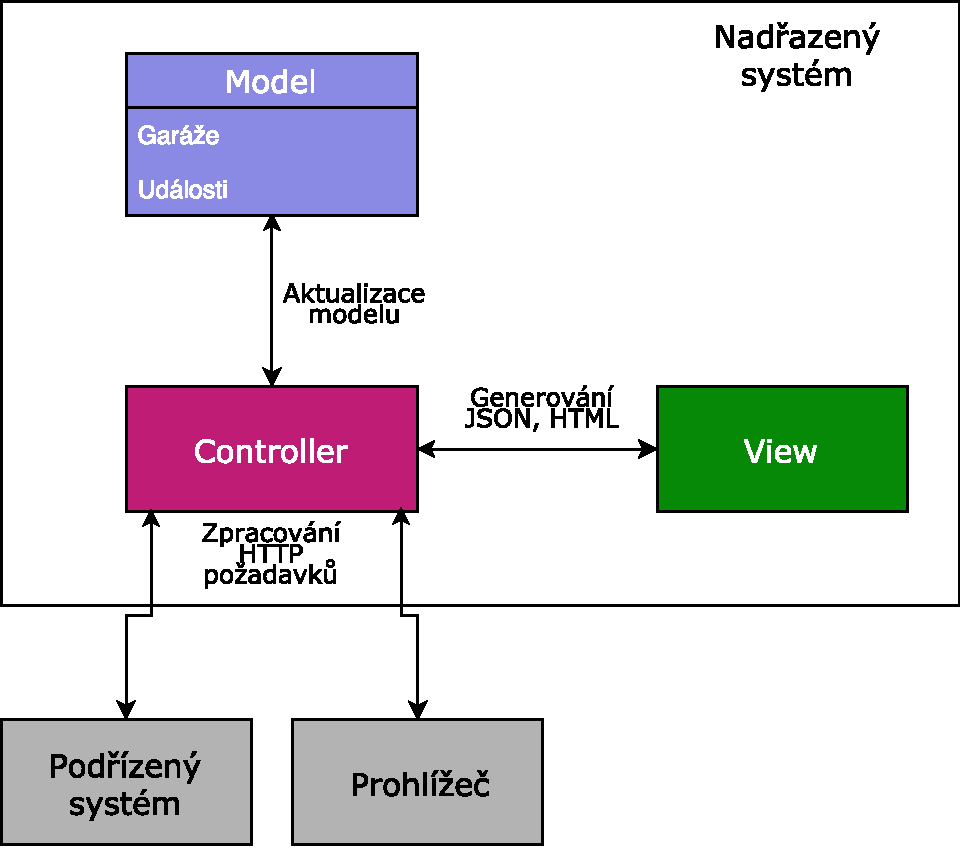
\includegraphics[width=0.7\textwidth]{images/mvc.pdf}
    \caption{Struktura MVC aplikace}
    \label{fig:mvc}
\end{figure}

Hlavní motivací pro použití tohoto vzoru je snadná rozšiřitelnost. Pokud by například bylo potřeba aplikaci doplnit o~komunikaci s~podřízenými systémy pomocí MQTT, stačí pouze vytvořit vhodný \textit{controller}. Ten pak může využívat \textit{model} aplikace stejným způsobem jako HTTP \textit{controller}.

\section{Model}

pouziti sqlalchemy -- to resit az v~implementaci

\subsection{Garáž}

\subsubsection{Stav garáže}

\subsection{Událost}

\subsubsection{Vyhodnocení události}

\subsection{Fasáda}

\section{Controller}

Flask API

\section{View}

\section{Autentizace}

\subsection{Autentizace uživatele}

\subsection{Autentizace podřízeného systému}

\subsubsection{Registrační mód}

